\documentclass{article}
\usepackage[margin=0.625in]{geometry}
\usepackage{tikz}
\usepackage{fourier}
\usepackage[scaled=0.85]{berasans}
\usepackage[scaled=0.85]{beramono}

\usepackage{fancyhdr}
\pagestyle{fancyplain} 
\fancyhead[co]{\textbf{\huge{Valid Syllogistic Forms}}}
\fancyfoot[l]{\tiny{Prepared using \LaTeX}}
\fancyfoot[r]{\textcopyright\tiny{\today Philip R. Huffman}}
\fancyfoot[c]{}

%set up row spacing
\def\rowa{0mm}
\def\rowb{-75mm}
\def\rowc{-150mm}
\def\rowd{-225mm}

%set up column spacing
\def\cola{0mm}
\def\colb{41mm}
\def\colc{82mm}
\def\cold{123mm}
\def\cole{164mm}
\def\colf{205mm}

%define the three circles that comprise a Venn diagram
\def\sCircle{(0,0) circle (11mm)}
\def\mCircle{(60:11mm) circle (11mm)}
\def\pCircle{(0:11mm) circle (11mm)}

%define the Venn diagram with labels
\def\venn{%
     \draw \sCircle; 
     \draw \mCircle; 
     \draw \pCircle;
     \draw (-0.9, -1.3) node{$S$};
     \draw (1.9, -1.3) node{$P$};
     \draw (0.5, 2.5) node{$M$};
}

%define x for zone 2
\def\zoneTwoX{%
    \draw [red] (-0.15,0.725) node{X};
}

%define circled x for zone 2
\def\zoneTwoCircX{%
    \zoneTwoX;
    \draw [red] (-0.15,0.725) circle(2.50mm);
}

%define x for zone 3
\def\zoneThreeX{%
    \draw [red] (0.55,0.33) node{X};
}

%define circled x for zone 3
\def\zoneThreeCircX{%
    \zoneThreeX;
    \draw [red] (0.55,0.33) circle(2.50mm);
}

%define x for zone 4
\def\zoneFourX{%
    \draw [red] (1.25,0.725) node{X};
}

%define circled x for zone 4
\def\zoneFourCircX{%
    \zoneFourX;
    \draw [red] (1.25,0.725) circle(2.50mm);
}

%define x for zone 5
\def\zoneFiveX{%
    \draw [red] (-0.55,-0.2) node{X};
}

%define circled x for zone 5
\def\zoneFiveCircX{%
    \zoneFiveX;
    \draw [red] (-0.55,-0.2) circle(3mm);
}

%define the fill color
\def\fillColor{red!40}

\begin{document}
    \begin{center}
%        \begin{huge}
%            Valid Syllogistic Forms\vspace{.25in}
%        \end{huge}

        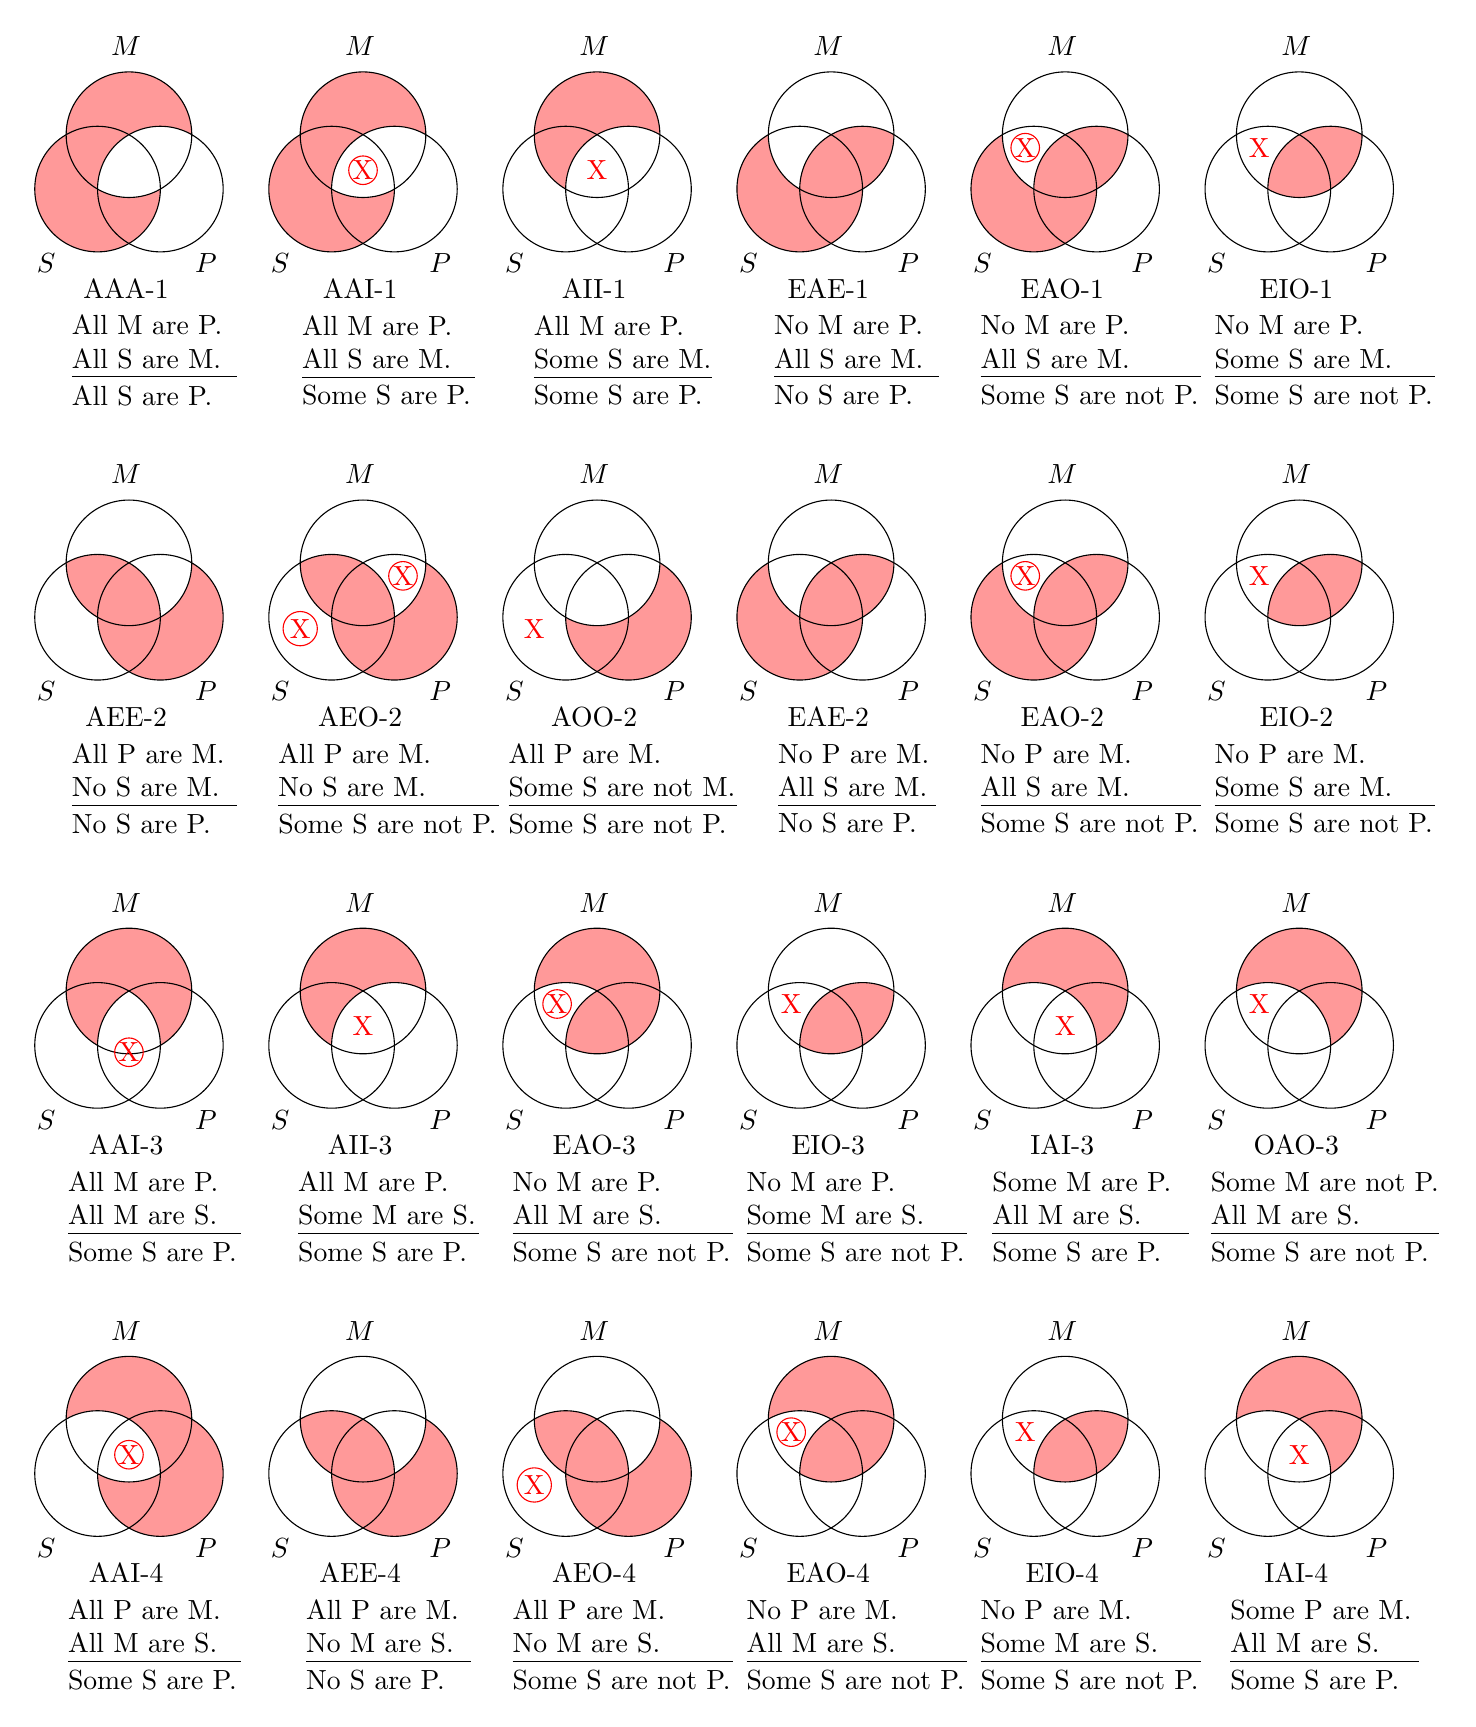
\begin{tikzpicture}[scale=0.725]
    %
    %AAA-1
            \begin{scope}[shift={(\cola, \rowa)}]
                \fill[\fillColor]\mCircle;
                \fill[\fillColor]\sCircle;
                \begin{scope}
                    \clip \mCircle;
                    \fill[white]\pCircle;
                \end{scope}
                \venn;
                \draw (.5,-1.75) node {AAA-1};
                \draw (1, -3) node[text width=21mm]{%
                    All M are P.\\
                    All S are M.\vspace{3pt}\\\hrule\vspace{3pt}
                    All S are P.
                };
            \end{scope}
    %
    %AAI-1
            \begin{scope}[shift={(\colb, \rowa)}]
                \fill[\fillColor]\mCircle;
                \fill[\fillColor]\sCircle;
                \begin{scope}
                    \clip \mCircle;
                    \fill[white]\pCircle;
                \end{scope}
                \venn;
                \draw (.5,-1.75) node {AAI-1};
                \draw (1, -3) node[text width=22mm]{%
                    All M are P.\\
                    All S are M.\vspace{3pt}\\\hrule\vspace{3pt}
                    Some S are P.
                };
                \zoneThreeCircX;
            \end{scope}
    %
    %AII-1
            \begin{scope}[shift={(\colc, \rowa)}]
                \fill[\fillColor]\mCircle;
                \fill[white]\pCircle;
                \venn;
                \draw (.5,-1.75) node {AII-1};
                \draw (1, -3) node[text width=22.6mm]{%
                    All M are P.\\
                    Some S are M.\vspace{3pt}\\\hrule\vspace{3pt}
                    Some S are P.
                };
                \zoneThreeX;
            \end{scope}
    %
    %EAE-1
            \begin{scope}[shift={(\cold, \rowa)}]
                \fill[\fillColor]\sCircle;
                \begin{scope}
                    \clip \mCircle;
                    \fill[white]\sCircle;
                \end{scope}
                \begin{scope}
                    \clip \pCircle;
                    \fill[\fillColor]\mCircle;
                \end{scope}
                \venn;
                \draw (.5,-1.75) node {EAE-1};
                \draw (1, -3) node[text width=21mm]{%
                    No M are P.\\
                    All S are M.\vspace{3pt}\\\hrule\vspace{3pt}
                    No S are P.
                };
            \end{scope}
    %
    %EAO-1
            \begin{scope}[shift={(\cole, \rowa)}]
                \fill[\fillColor]\sCircle;
                \begin{scope}
                    \clip \mCircle;
                    \fill[white]\sCircle;
                \end{scope}
                \begin{scope}
                    \clip \pCircle;
                    \fill[\fillColor]\mCircle;
                \end{scope}
                \venn;
                \draw (.5,-1.75) node {EAO-1};
                \draw (1, -3) node[text width=28mm]{%
                    No M are P.\\
                    All S are M.\vspace{3pt}\\\hrule\vspace{3pt}
                    Some S are not P.
                };
                \zoneTwoCircX;
            \end{scope}
    %
    %EIO-1
            \begin{scope}[shift={(\colf, \rowa)}]
                \begin{scope}
                    \clip \pCircle;
                    \fill[\fillColor]\mCircle;
                \end{scope}
                \venn;
                \draw (.5,-1.75) node {EIO-1};
                \draw (1, -3) node[text width=28mm]{%
                    No M are P.\\
                    Some S are M.\vspace{3pt}\\\hrule\vspace{3pt}
                    Some S are not P.
                };
                \zoneTwoX
            \end{scope}
    %
    %AEE-2
            \begin{scope}[shift={(\cola, \rowb)}]
                \fill[\fillColor]\pCircle;
                \fill[white]\mCircle;
                \begin{scope}
                    \clip \mCircle;
                    \fill[\fillColor]\sCircle;
                \end{scope}
                \venn;
                \draw (.5,-1.75) node {AEE-2};
                \draw (1, -3) node[text width=21mm]{%
                    All P are M.\\
                    No S are M.\vspace{3pt}\\\hrule\vspace{3pt}
                    No S are P.
                };
            \end{scope}
    %
    %AEO-2
            \begin{scope}[shift={(\colb, \rowb)}]
                \fill[\fillColor]\pCircle;
                \fill[white]\mCircle;
                \begin{scope}
                    \clip \mCircle;
                    \fill[\fillColor]\sCircle;
                \end{scope}
                \venn;
                \draw (.5,-1.75) node {AEO-2};
                \draw (1, -3) node[text width=28mm]{%
                    All P are M.\\
                    No S are M.\vspace{3pt}\\\hrule\vspace{3pt}
                    Some S are not P.
                };
                \zoneFourCircX;
                \zoneFiveCircX;
            \end{scope}
    %
    %AOO-2
            \begin{scope}[shift={(\colc, \rowb)}]
                \fill[\fillColor]\pCircle;
                \fill[white]\mCircle;
                \venn;
                \zoneFiveX;
                \draw (.5,-1.75) node {AOO-2};
                \draw (1, -3) node[text width=29mm]{%
                    All P are M.\\
                    Some S are not M.\vspace{3pt}\\\hrule\vspace{3pt}
                    Some S are not P.
                };
            \end{scope}
    %
    %EAE-2
            \begin{scope}[shift={(\cold, \rowb)}]
                \fill[\fillColor]\sCircle;
                \begin{scope}
                    \clip \sCircle;
                    \fill[white]\mCircle;
                \end{scope}
                \begin{scope}
                    \clip \pCircle;
                    \fill[\fillColor]\mCircle;
                \end{scope}
                \venn;
                \draw (.5,-1.75) node {EAE-2};
                \draw (1, -3) node[text width=20mm]{%
                    No P are M.\\
                    All S are M.\vspace{3pt}\\\hrule\vspace{3pt}
                    No S are P.
                };
            \end{scope}
    %
    %EAO-2
            \begin{scope}[shift={(\cole, \rowb)}]
                \fill[\fillColor]\sCircle;
                \begin{scope}
                    \clip \sCircle;
                    \fill[white]\mCircle;
                \end{scope}
                \begin{scope}
                    \clip \pCircle;
                    \fill[\fillColor]\mCircle;
                \end{scope}
                \venn;
                \draw (.5,-1.75) node {EAO-2};
                \draw (1, -3) node[text width=28mm]{%
                    No P are M.\\
                    All S are M.\vspace{3pt}\\\hrule\vspace{3pt}
                    Some S are not P.
                };
                \zoneTwoCircX;
            \end{scope}
    %
    %EIO-2
            \begin{scope}[shift={(\colf, \rowb)}]
                \begin{scope}
                    \clip \pCircle;
                    \fill[\fillColor]\mCircle;
                \end{scope}
                \venn;
                \draw (.5,-1.75) node {EIO-2};
                \draw (1, -3) node[text width=28mm]{%
                    No P are M.\\
                    Some S are M.\vspace{3pt}\\\hrule\vspace{3pt}
                    Some S are not P.
                };
                \zoneTwoX;
            \end{scope}
    %
    %AAI-3
            \begin{scope}[shift={(\cola, \rowc)}]
                \fill[\fillColor]\mCircle;
                \begin{scope}
                    \clip \sCircle;
                    \clip \mCircle;
                    \clip \pCircle;
                    \fill[white]\mCircle;
                \end{scope}
                \venn;
                \draw (.5,-1.75) node {AAI-3};
                \draw (1, -3) node[text width=22mm]{%
                    All M are P.\\
                    All M are S.\vspace{3pt}\\\hrule\vspace{3pt}
                    Some S are P.
                };
                \begin{scope}[shift={(0mm,-4.5mm)}]
                    \zoneThreeCircX;
                \end{scope}
            \end{scope}
    %
    %AII-3
            \begin{scope}[shift={(\colb, \rowc)}]
                \fill[\fillColor]\mCircle;
                \fill[white]\pCircle;
                \venn;
                \draw (.5,-1.75) node {AII-3};
                \draw (1, -3) node[text width=23mm]{%
                    All M are P.\\
                    Some M are S.\vspace{3pt}\\\hrule\vspace{3pt}
                    Some S are P.
                };
                \zoneThreeX;
            \end{scope}
    %
    %EAO-3
            \begin{scope}[shift={(\colc, \rowc)}]
                \fill[\fillColor]\mCircle;
                \begin{scope}
                    \clip \sCircle;
                    \clip \mCircle;
                    \fill[white]\sCircle;
                    \clip \pCircle;
                    \fill [\fillColor]\pCircle;
                \end{scope}
                \venn;
                \draw (.5,-1.75) node {EAO-3};
                \draw (1, -3) node[text width=28mm]{%
                    No M are P.\\
                    All M are S.\vspace{3pt}\\\hrule\vspace{3pt}
                    Some S are not P.
                };
                \zoneTwoCircX;
            \end{scope}
    %
    %EIO-3
            \begin{scope}[shift={(\cold, \rowc)}]
                \begin{scope}
                    \clip \pCircle;
                    \fill[\fillColor]\mCircle;
                \end{scope}
                \venn;
                \draw (.5,-1.75) node {EIO-3};
                \draw (1, -3) node[text width=28mm]{%
                    No M are P.\\
                    Some M are S.\vspace{3pt}\\\hrule\vspace{3pt}
                    Some S are not P.
                };
                \zoneTwoX;
            \end{scope}
    %
    %IAI-3
            \begin{scope}[shift={(\cole, \rowc)}]
                \fill[\fillColor]\mCircle;
                \begin{scope}
                    \clip \sCircle;
                    \fill[white]\mCircle;
                    \draw [red] (.55,0.333) node{X};
                \end{scope}
                \venn;
                \draw (.5,-1.75) node {IAI-3};
                \draw (1, -3) node[text width=25mm]{%
                    Some M are P.\\
                    All M are S.\vspace{3pt}\\\hrule\vspace{3pt}
                    Some S are P.
                };
            \end{scope}
    %
    %OAO-3
            \begin{scope}[shift={(\colf, \rowc)}]
                \fill[\fillColor]\mCircle;
                \begin{scope}
                    \clip \sCircle;
                    \fill[white]\mCircle;
                \end{scope}
                \venn;
                \draw (.5,-1.75) node {OAO-3};
                \draw (1, -3) node[text width=29mm]{%
                    Some M are not P.\\
                    All M are S.\vspace{3pt}\\\hrule\vspace{3pt}
                    Some S are not P.
                };
                \zoneTwoX;
            \end{scope}
    %
    %AAI-4
            \begin{scope}[shift={(\cola, \rowd)}]
                \fill[\fillColor]\mCircle;
                \fill[\fillColor]\pCircle;
                \begin{scope}
                    \clip \mCircle;
                    \fill[white]\sCircle;
               \end{scope}
                \venn;
                \draw (.5,-1.75) node {AAI-4};
                \draw (1, -3) node[text width=22mm]{%
                    All P are M.\\
                    All M are S.\vspace{3pt}\\\hrule\vspace{3pt}
                    Some S are P.
                };
                \zoneThreeCircX;
            \end{scope}
    %
    %AEE-4
            \begin{scope}[shift={(\colb, \rowd)}]
                \fill[\fillColor]\pCircle;
                \fill[white]\mCircle;
                \begin{scope}
                    \clip \sCircle;
                    \fill[\fillColor]\mCircle;
               \end{scope}
                \venn;
                \draw (.5,-1.75) node {AEE-4};
                \draw (1, -3) node[text width=21mm]{%
                    All P are M.\\
                    No M are S.\vspace{3pt}\\\hrule\vspace{3pt}
                    No S are P.
                };
            \end{scope}
    %
    %AEO-4
            \begin{scope}[shift={(\colc, \rowd)}]
                \fill[\fillColor]\pCircle;
                \fill[white]\mCircle;
                \begin{scope}
                    \clip \sCircle;
                    \fill[\fillColor]\mCircle;
                \end{scope}
                \venn;
                \draw (.5,-1.75) node {AEO-4};
                \draw (1, -3) node[text width=28mm]{%
                    All P are M.\\
                    No M are S.\vspace{3pt}\\\hrule\vspace{3pt}
                    Some S are not P.
                };
                \zoneFiveCircX;
            \end{scope}
    %
    %EAO-4
            \begin{scope}[shift={(\cold, \rowd)}]
                \fill[\fillColor]\mCircle;
                \begin{scope}
                    \clip \sCircle;
                    \fill[white]\mCircle;
                \end{scope}
                \begin{scope}
                    \clip \sCircle;
                    \clip \mCircle;
                    \clip \pCircle;
                    \fill[\fillColor]\mCircle;
                \end{scope}
                \venn;
                \draw (.5,-1.75) node {EAO-4};
                \draw (1, -3) node[text width=28mm]{%
                    No P are M.\\
                    All M are S.\vspace{3pt}\\\hrule\vspace{3pt}
                    Some S are not P.
                };
                \zoneTwoCircX;
            \end{scope}
    %
    %EIO-4
            \begin{scope}[shift={(\cole, \rowd)}]
                \begin{scope}
                    \clip \mCircle;
                    \fill[\fillColor]\pCircle;
                \end{scope}
                \venn;
                \draw (.5,-1.75) node {EIO-4};
                \draw (1, -3) node[text width=28mm]{%
                    No P are M.\\
                    Some M are S.\vspace{3pt}\\\hrule\vspace{3pt}
                    Some S are not P.
                };
                \zoneTwoX;
            \end{scope}
    %
    %IAI-4
            \begin{scope}[shift={(\colf, \rowd)}]
                \fill[\fillColor]\mCircle;
                \fill[white]\sCircle;
                \venn;
                \draw (.5,-1.75) node {IAI-4};
                \draw (1, -3) node[text width=24mm]{%
                    Some P are M.\\
                    All M are S.\vspace{3pt}\\\hrule\vspace{3pt}
                    Some S are P.
                };
                \zoneThreeX;
            \end{scope}
        \end{tikzpicture}
    \end{center}
\end{document}